\documentclass[a4paper]{article}
\usepackage[utf8]{inputenc}
\usepackage[czech]{babel}
\usepackage[margin=13mm, tmargin=15mm, bmargin=12mm]{geometry}
\usepackage{multirow}
\usepackage{tikz}
\usetikzlibrary{calc}
\usepackage{chngpage}
\usepackage{tabularx}
\usepackage{fancyhdr}
\usepackage{mathptmx}
\usepackage{siunitx}
\usepackage{float}
\usepackage{longtable}
\usepackage{hyperref}
\usepackage{subcaption}

\sisetup{
	round-mode = places,
	round-precision = 4,
	round-pad = false
}

\renewcommand{\baselinestretch}{1.15}
\pagenumbering{gobble}
\pagestyle{fancy}
\renewcommand{\headrulewidth}{0pt}

\newcommand{\jmeno}{David Škrob, Tom\'{a}\v{s} N\'{a}zler}
\newcommand{\trida}{L4A}
\newcommand{\poradovecislo}{}
\newcommand{\nazevulohy}{Transformatory}
\newcommand{\cisloulohy}{}
\newcommand{\predmet}{Technické měření}
\newcommand{\skupina}{}
\newcommand{\datummereni}{22.9.2022}
\newcommand{\datumodevzdani}{2.10.2022}
\newcommand{\klasifikace}{}
\begin{document}
\fancyhead{
\begin{tikzpicture} [overlay,remember picture]
       \draw
        ($ (current page.north west) + (1cm, -12mm) $)
        rectangle
        ($ (current page.south east) + (-1cm,12mm) $);
\end{tikzpicture}
}

\renewcommand{\arraystretch}{2}
\shorthandoff{-}

{
\begin{adjustwidth}[]{-3mm}{-3mm}
\centering
\vspace*{-7mm}
\begin{tabularx}{\linewidth}{l|X|p{3cm}}
\multirow{2}{25mm}{\centering SPŠ a VOŠ technická Brno, Sokolská 1} &
\textbf{LABORATORNÍ CVIČENÍ Z ELEKTROTECHNIKY} & Třída: \trida \\
\cline{2-3}
 & Jméno a příjmení: \jmeno & Poř. Číslo: \poradovecislo \\
\hline
\end{tabularx}

\begin{tabularx}{\linewidth}{X|p{3cm}}
Název úlohy: \nazevulohy & Číslo úlohy: \cisloulohy \\
\hline
Zkoušený předmět: \predmet & Skupina: \skupina \\
\hline
\end{tabularx}

\begin{tabularx}{\linewidth}{X|X|X}
Datum měření: \datummereni &  Datum odevzdání: \datumodevzdani &  Klasifikace: \klasifikace \\
\hline
\end{tabularx}

\end{adjustwidth}
}

\shorthandon{-}
\section*{Teorie}
\subsection*{Transform\'ator napr\'{a}zdno}
Jeho sekund\'arn\'i vinut\'i nen\'i zapojeno na \v{z}\'adn\'y spot\v{r}ebi\v{c} - transform\'ator ned\'ava v\'ykon. V\v{e}t\v{s}ina p\v{r}\'ykonu jde do zmagnetov\'an\'i j\'adra, proto \v{r}\'ik\'ame t\v{e}mto ztr\'atam, \textbf{ztr\'aty v \v{z}eleze} 
\subsection*{Transform\'ator nakr\'{a}tko}
Jeho sekund\'arn\'i vinut\'i je zapojeno do zkratu.
Proud je mnohon\'asobn\v{e} v\v{e}t\v{s}\'i - Tepeln\'e ztr\'aty rostou s druhou odmocninou proudu.
Magnetick\'e toky jsou mal\'e, ztr\'aty v magnetick\'em obvodu (v\'i\v{r}iv\'e proudy) jsou zanedbateln\'e. Proto se ztr\'aty nakr\'atko tak\'e naz\'yvaj\'i \textbf{ztr\'aty v m\v{e}di}.
\subsection*{Vzorce}
Pro \v{c}inn\'y v\'ykon $P$, jalov\'y v\'ykon $Q$, zd\'anliv\'y v\'ykon S:
\begin{equation}\label{vykon}
	P = U I \cos \varphi
\end{equation}
\begin{equation}\label{prikon}
	Q = U I \sin \varphi
\end{equation}
\begin{equation}\label{zdanlivy}
	S=\sqrt{Q^2+P^2}
\end{equation}
Kde $U$ a $I$ jsou efektivn\'i hodnoty.\\
F\'azi $\varphi$ vypo\v{c}\'itame dle:
\begin{equation}
	\frac{\Delta t}{T} = \frac{\varphi}{2\pi}
\end{equation}
Kde $\Delta t$ je \v{c}asov\'y posun proudu vů\v{c}i nap\v{e}t\'i
\section*{Zadání}
Zm\v{e}\v{r}te:
\begin{enumerate}
	\item \begin{enumerate}
		\item Pr\r{u}b\v{e}h nap\v{e}t\'i a proudu v prim\'arn\'im vinut\'i transform\'atoru \underline{nakr\'atko} - vytvo\v{r}te graf
		\item \label{1b} Nap\v{e}t\'i, proud a f\'azov\'y posun transform\'atoru nakr\'atko pro tyto kombinace hodnot: $U$ = \SI{1}{\volt} a \SI{2}{\volt}, $f$ = \SI{50}{\hertz} a \SI{100}{\hertz}, vypo\v{c}t\v{e}te v\'ykony $P$,$Q$,$S$ - vytvo\v{r}te tabulku
	\end{enumerate}
	\item \begin{enumerate}
		\item Pr\r{u}b\v{e}h nap\v{e}t\'i a proudu v prim\'arn\'im vinut\'i transform\'atoru \underline{napr\'azdno} - vytvo\v{r}te graf
		\item  \label{2b} Nap\v{e}t\'i, proud a f\'azov\'y posun transform\'atoru napr\'azdno pro tyto kombinace hodnot: $U$ = \SI{1}{\volt} a \SI{2}{\volt}, $f$ = \SI{50}{\hertz} a \SI{100}{\hertz}, vypo\v{c}t\v{e}te v\'ykony $P$,$Q$,$S$ - vytvo\v{r}te tabulku
	\end{enumerate}
	\item \begin{enumerate}
		\item Pr\r{u}b\v{e}h nap\v{e}t\'i a proudu v prim\'arn\'im vinut\'i \underline{zat\'i\v{z}eneho} transformatoru - vytvo\v{r}te graf
		\item \label{3b} Nap\v{e}t\'i, proud a f\'azov\'y posun zat\'i\v{z}eneho transform\'atoru pro tyto kombinace hodnot: $U$ = \SI{1}{\volt} a \SI{2}{\volt}, $f$ = \SI{50}{\hertz} a \SI{100}{\hertz}, vypo\v{c}t\v{e}te v\'ykony $P$,$Q$,$S$ - vytvo\v{r}te tabulku
	\end{enumerate}
	\item \label{4} Nap\v{e}t\'i v prim\'arn\'im vinut\'i napr\'azdno - vytvo\v{r}te graf + porovn\'an\'i teoretick\'e hodnoty $U_2$ se skute\v{c}nou. Nap\v{e}t\'i na zdroji nastavte na \SI{5}{\volt}, \SI{100}{\hertz}.
	\item \label{5} Proud v prim\'arn\'im vinut\'i a sekund\'arn\'im nakr\'atko – vytvo\v{r}te graf + porovn\'an\'i teoretick\'e hodnoty $I_2$ se skute\v{c}nou. Nap\v{e}t\'i na zdroji nastavte na \SI{300}{\milli\volt} \SI{100}{\hertz}.\\
\end{enumerate}
\section*{Vypracování}
\begin{figure}[h!]
	\centering
	\begin{subfigure}{0.49\textwidth}
		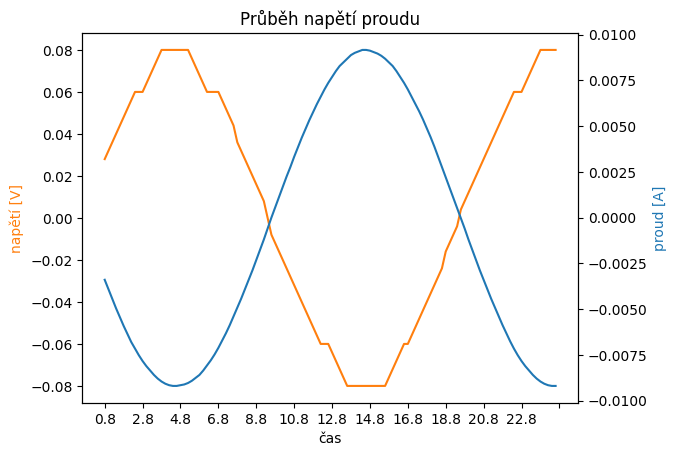
\includegraphics[width=\textwidth]{Trafo1b_1V.png}
		\caption{Transformátor při napětí \SI{1}{\volt} a frekvenci \SI{50}{\hertz}}
	\end{subfigure}
	\hfill
	\begin{subfigure}{0.49\textwidth}
		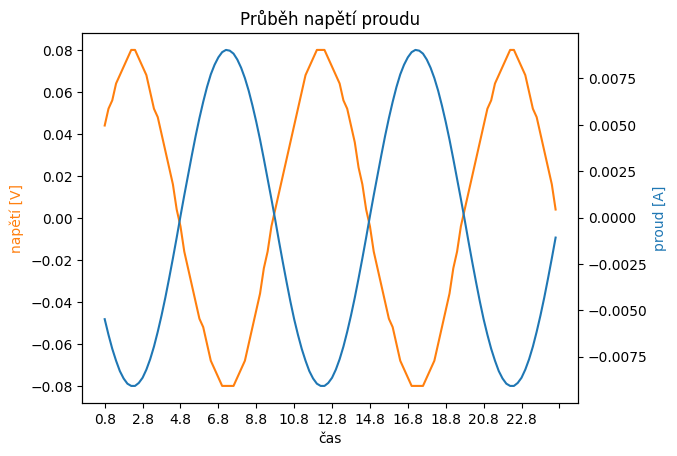
\includegraphics[width=\textwidth]{Trafo1b_1V_100Hz.png}
		\caption{Transformátor při napětí \SI{1}{\volt} a frekvenci \SI{100}{\hertz}}
	\end{subfigure}
	\hfill
	\begin{subfigure}{0.49\textwidth}
		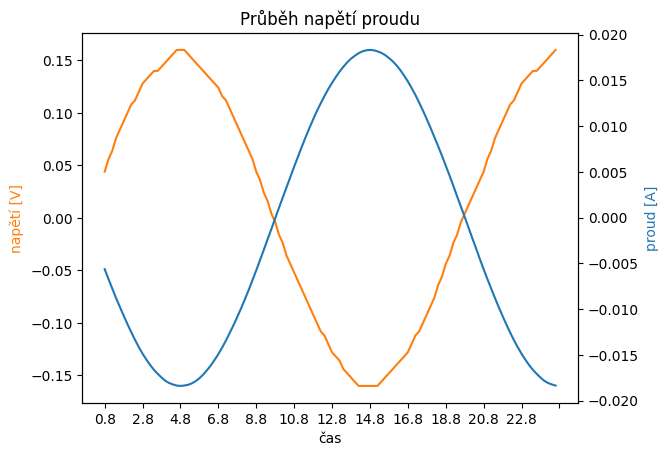
\includegraphics[width=\textwidth]{Trafo1b_2V_50Hz.png}
		\caption{Transformátor při napětí \SI{2}{\volt} a frekvenci \SI{50}{\hertz}}
	\end{subfigure}
	\hfill
	\begin{subfigure}{0.49\textwidth}
		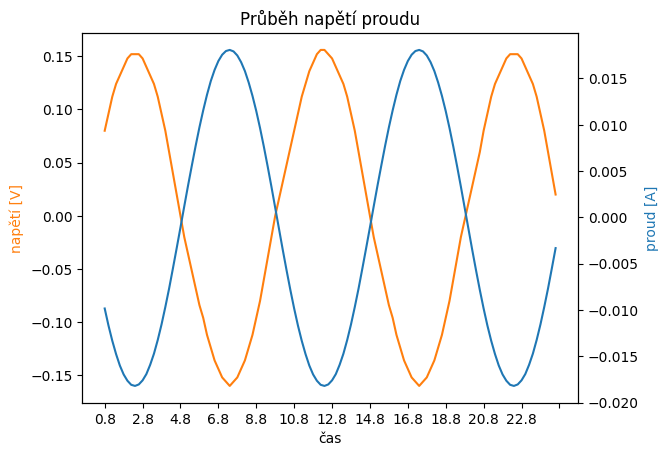
\includegraphics[width=\textwidth]{Trafo1b_2V_100Hz.png}
		\caption{Transformátor při napětí \SI{2}{\volt} a frekvenci \SI{100}{\hertz}}
	\end{subfigure}
	\caption{Grafy vztahující se k úloze \ref{1b}}
\end{figure}

\begin{figure}[h!]
	\centering
	\begin{subfigure}{0.49\textwidth}
		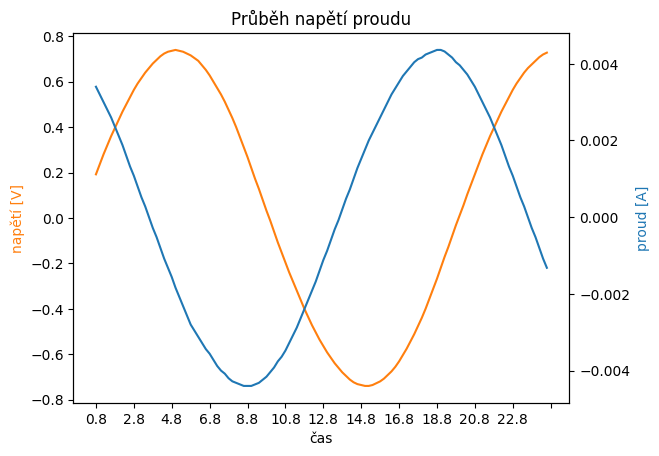
\includegraphics[width=\textwidth]{Trafo2b_1V_50Hz.png}
		\caption{Transformátor při napětí \SI{1}{\volt} a frekvenci \SI{50}{\hertz}}
	\end{subfigure}
	\hfill
	\begin{subfigure}{0.49\textwidth}
		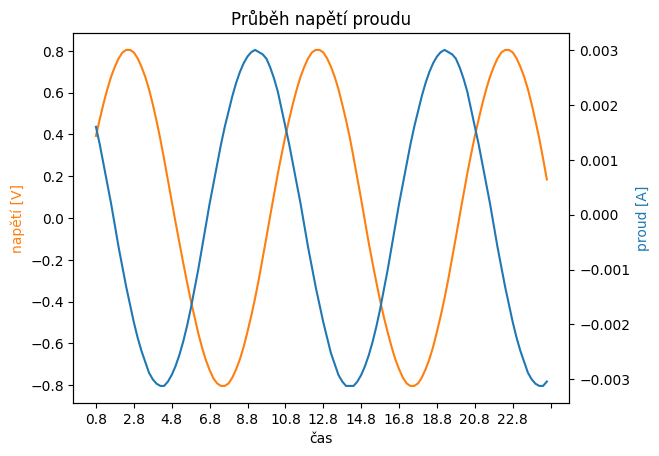
\includegraphics[width=\textwidth]{Trafo2b_1V_100Hz.png}
		\caption{Transformátor při napětí \SI{1}{\volt} a frekvenci \SI{100}{\hertz}}
	\end{subfigure}
	\hfill
	\begin{subfigure}{0.49\textwidth}
		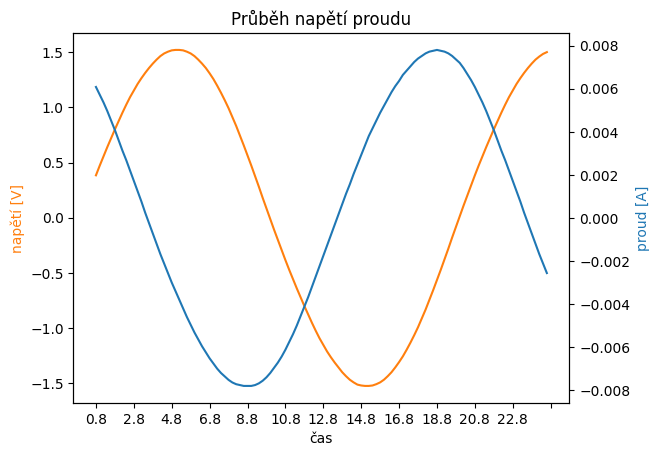
\includegraphics[width=\textwidth]{Trafo2b_2V_50Hz.png}
		\caption{Transformátor při napětí \SI{2}{\volt} a frekvenci \SI{50}{\hertz}}
	\end{subfigure}
	\hfill
	\begin{subfigure}{0.49\textwidth}
		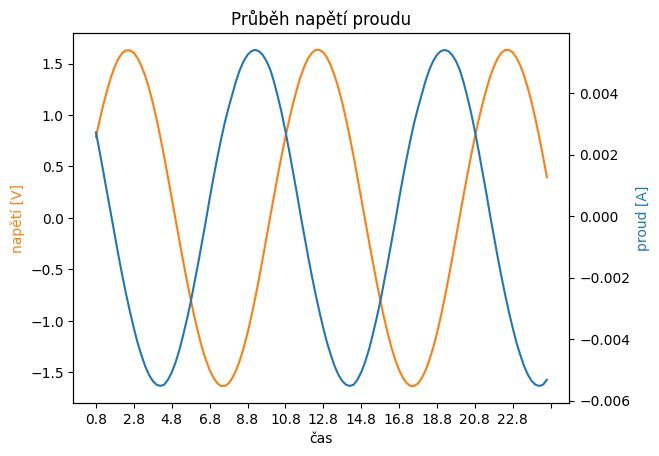
\includegraphics[width=\textwidth]{Trafo2b_2V_100Hz.png}
		\caption{Transformátor při napětí \SI{2}{\volt} a frekvenci \SI{100}{\hertz}}
	\end{subfigure}
	\caption{Grafy vztahující se k úloze \ref{2b}}
\end{figure}

\begin{figure}[h!]
	\centering
	\begin{subfigure}{0.49\textwidth}
		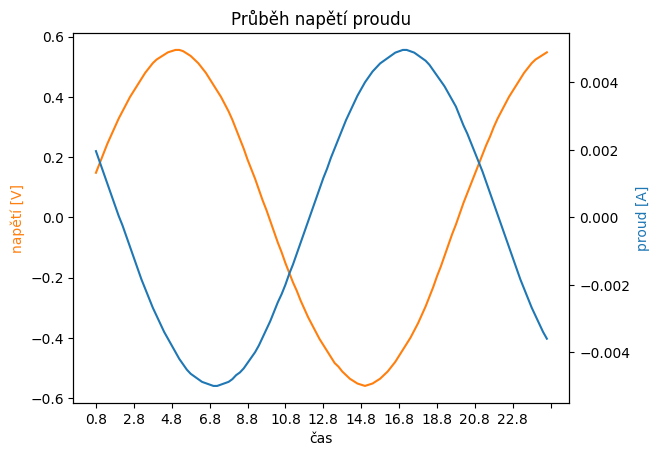
\includegraphics[width=\textwidth]{Trafo3b_1V_50Hz.png}
		\caption{Transformátor při napětí \SI{1}{\volt} a frekvenci \SI{50}{\hertz}}
	\end{subfigure}
	\hfill
	\begin{subfigure}{0.49\textwidth}
		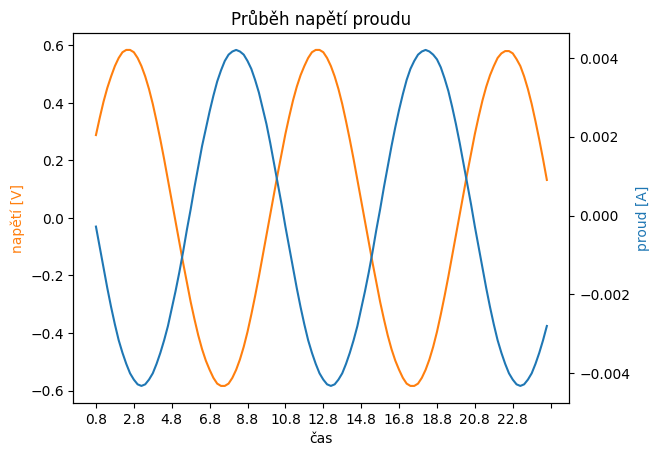
\includegraphics[width=\textwidth]{Trafo3b_1V_100Hz.png}
		\caption{Transformátor při napětí \SI{1}{\volt} a frekvenci \SI{100}{\hertz}}
	\end{subfigure}
	\hfill
	\begin{subfigure}{0.49\textwidth}
		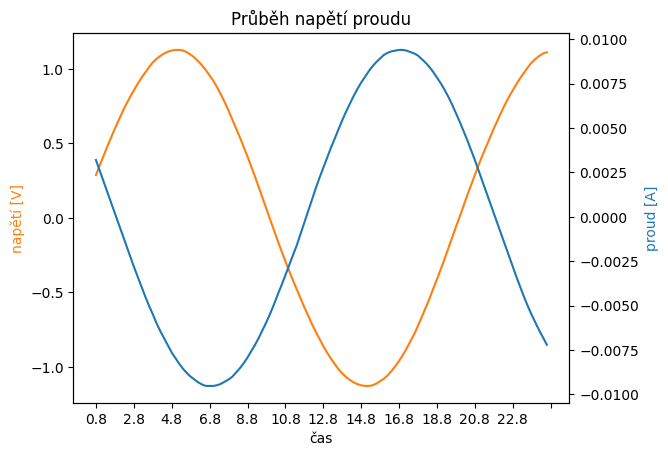
\includegraphics[width=\textwidth]{Trafo3b_2V_50Hz.png}
		\caption{Transformátor při napětí \SI{2}{\volt} a frekvenci \SI{50}{\hertz}}
	\end{subfigure}
	\hfill
	\begin{subfigure}{0.49\textwidth}
		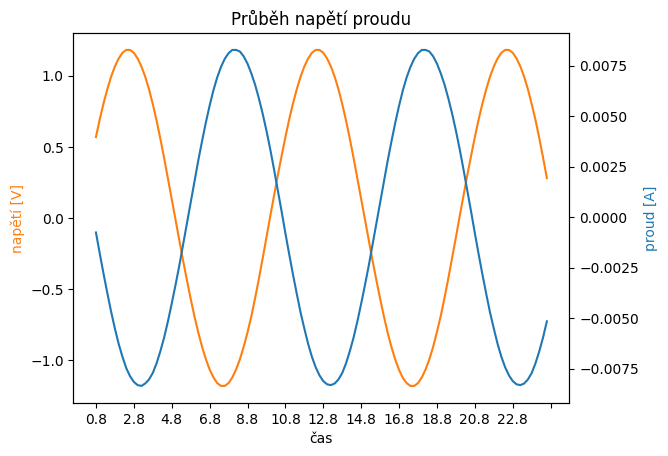
\includegraphics[width=\textwidth]{Trafo3b_2V_100Hz.png}
		\caption{Transformátor při napětí \SI{2}{\volt} a frekvenci \SI{100}{\hertz}}
	\end{subfigure}
	\caption{Grafy vztahující se k úloze \ref{3b}}
\end{figure}

\begin{figure}[h!]
	\centering
	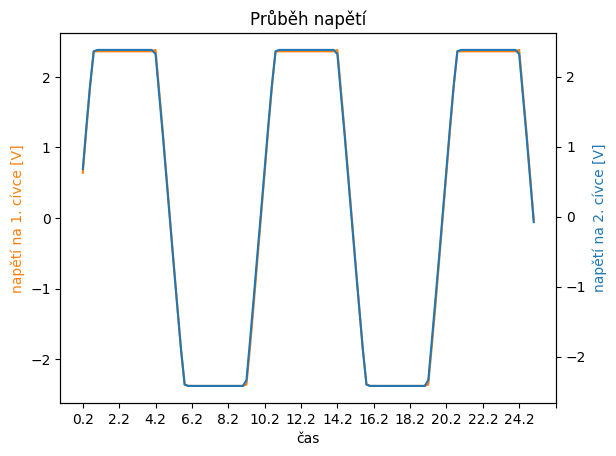
\includegraphics[width=0.6\linewidth]{Trafo4_5V_100Hz.png}
	\caption{Graf k úloze \ref{4}}
\end{figure}

\begin{figure}[h!]
	\centering
	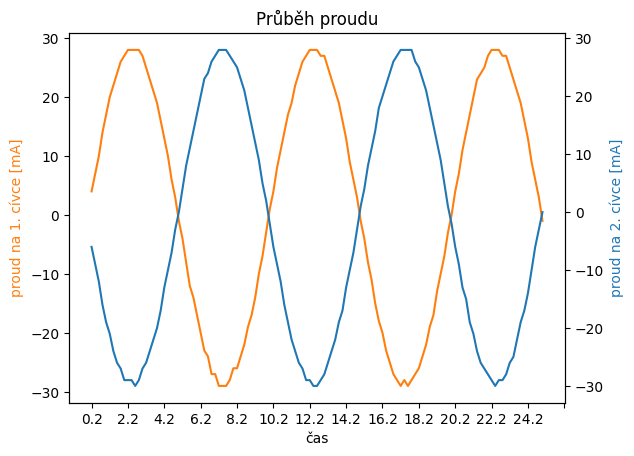
\includegraphics[width=0.6\linewidth]{Trafo5_300mV_100Hz.png}
	\caption{Graf k úloze \ref{5}}
\end{figure}

\begin{table}[!ht]
	\centering
	\begin{tabular}{|l|l|l|l|l|l|l|l|l|}
		\hline
		úloha & fáze [rad] & $I_{max}$ [\SI{}{\ampere}] & $U_{max}$ [\SI{}{\volt}]& $I$ [\SI{}{\ampere}]& $U$ [\SI{}{\volt}]& $P$ [\SI{}{\watt}]&$ Q$ [\SI{}{\watt}]
		& $S$ [\SI{}{\watt}]\\ \hline
		1b: \SI{1}{\volt}, \SI{50}{\hertz}&\num{3.14159}&\num{0.0092}&\num{0.08}&\num{0.0065053824}&\num{0.0565685425}&\num{-0.000368}&\num{0.000000001}&\num{0.000368} \\ \hline
		1b: \SI{1}{\volt}, \SI{100}{\hertz}&\num{3.14159}&\num{0.0092}&\num{0.08}&\num{0.0065053824}&\num{0.0565685425}&\num{-0.000368}&\num{0.000000001}&\num{0.000368} \\ \hline
		1b: \SI{2}{\volt}, \SI{50}{\hertz}&\num{3.14159}&\num{0.0184}&\num{0.16}&\num{0.0130107648}&\num{0.113137085}&\num{-0.001472}&\num{3.90608417581522E-009}&\num{0.001472} \\ \hline
		1b: \SI{2}{\volt}, \SI{100}{\hertz}&\num{3.14159}&\num{0.0184}&\num{0.16}&\num{0.0130107648}&\num{0.113137085}&\num{-0.001472}&\num{3.90608417581522E-009}&\num{0.001472} \\ \hline
		2b: \SI{1}{\volt}, \SI{50}{\hertz}&\num{2.0512653061}&\num{0.0044}&\num{0.74}&\num{0.0031112698}&\num{0.5232590181}&\num{-0.0007524536}&\num{0.001443675}&\num{0.001628} \\ \hline
		2b: \SI{1}{\volt}, \SI{100}{\hertz}&\num{2.094}&\num{0.003}&\num{0.82}&\num{0.0021213203}&\num{0.5798275606}&\num{-0.0006145791}&\num{0.0010654542}&\num{0.00123} \\ \hline
		2b: \SI{2}{\volt}, \SI{50}{\hertz}&\num{2.3440298507}&\num{0.0078}&\num{1.52}&\num{0.0055154329}&\num{1.0748023074}&\num{-0.0041404292}&\num{0.0042424085}&\num{0.005928} \\ \hline
		2b: \SI{2}{\volt}, \SI{100}{\hertz}&\num{2.094}&\num{0.0054}&\num{1.66}&\num{0.0038183766}&\num{1.1737972568}&\num{-0.0022394662}&\num{0.003882411}&\num{0.004482} \\ \hline
		3b: \SI{1}{\volt}, \SI{50}{\hertz}&\num{2.4999795918}&\num{0.005}&\num{0.56}&\num{0.0035355339}&\num{0.3959797975}&\num{-0.001121584}&\num{0.0008378839}&\num{0.0014} \\ \hline
		3b: \SI{1}{\volt}, \SI{100}{\hertz}&\num{2.748375}&\num{0.0042}&\num{0.6}&\num{0.0029698485}&\num{0.4242640687}&\num{-0.001163838}&\num{0.0004827847}&\num{0.00126} \\ \hline
		3b: \SI{2}{\volt}, \SI{50}{\hertz}&\num{2.5640816327}&\num{0.0094}&\num{1.14}&\num{0.0066468037}&\num{0.8061017306}&\num{-0.0044890614}&\num{0.0029251481}&\num{0.005358} \\ \hline
		3b: \SI{2}{\volt}, \SI{100}{\hertz}&\num{2.748375}&\num{0.0094}&\num{1.14}&\num{0.0066468037}&\num{0.8061017306}&\num{-0.0049490826}&\num{0.0020529846}&\num{0.005358} \\ \hline
	\end{tabular}
	\caption{tabulka všech hodnot z měření}
\end{table}
\clearpage

\section*{Závěr}
Transformátory se chovali dle našich předpokladů, z vytvořených grafů jsme si mohli ověřit teorii o fázovém posunu na cívkách.
 Co se týče hodnot výkonů a fází tak jsme použili poměrovou metodu která se nám zdála býti přehlednější a umožnila automatizaci.
Při měření napětí (úloha \ref{4}) jsme měli velkou odchylku měření, tak jsme nesrovnávali naměřené hodnoty s teoretickými. Měření proudu nám vyšlo přesně dle teorie.
%\vfill
\section*{Použité pomucky:}
\begin{tabularx}{\linewidth}{c|c|c|l}
	Přístroj – pomůcka&Typ&Rozsah (pouze analogové)
	& Poznámka \\
	\hline
	RLC 2000&&&\\
	\hline
	Transformator na RLC 2000&&&\\
	\hline
\end{tabularx}
\end{document}